\begin{answer}
\begin{figure}[h]
    \begin{subfigure}[b]{0.5\linewidth}
        \centering
        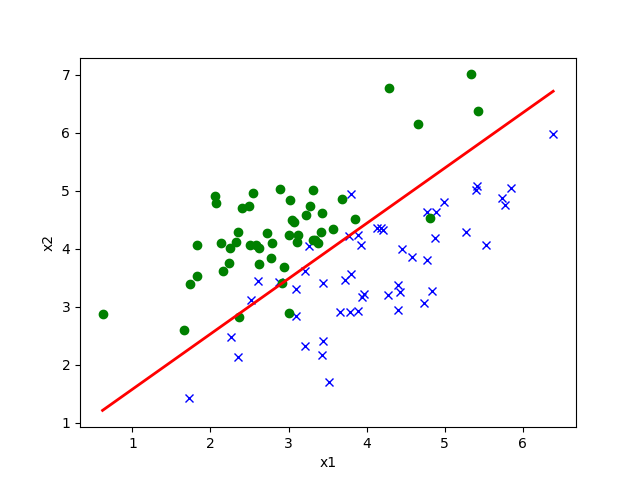
\includegraphics[width=\linewidth]{tex/p01b_pred_2.txt.png}
        \subcaption{Logistic Regression on Dataset 2}
    \end{subfigure}
    \begin{subfigure}[b]{0.5\linewidth}
        \centering
        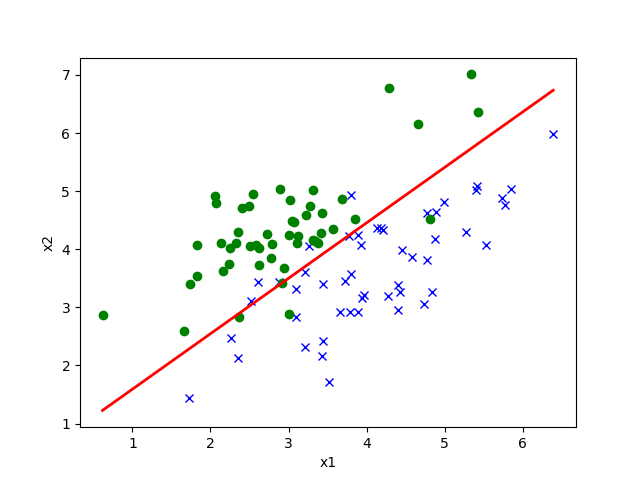
\includegraphics[width=\linewidth]{tex/p01e_pred_2.txt.png}
        \subcaption{GDA on Dataset 2}
    \end{subfigure}
\end{figure}
\\
GDA seems to perform worse than logistic regression on Dataset1, because the data distribution of Dataset1 is not like Guassian distribution.
\end{answer}
